\chapter{Tyranid Delivery}

\begin{wrapfigure}{O}{\figwidth}
	\begin{center}
		
\includegraphics[width=\figwidth]{pics/14/1.png}
	\end{center}
\end{wrapfigure}
Sarge glared out the window at the massive bulk of Way Station Alumentum Primaris. 
When he'd started the meeting it'd been a speck of light floating next to a marble-sized gas giant, but over the last hour it had grown into something that looked like a sort of jagged spinning top, and now it was a looming pile of gothic architecture studded with hangars, umbilicals, and a few massive docking arms. 
At this distance it looked a lot like a hive that had been lifted into space, which was rather disturbing since, after a lot of arguing between the Captain, Ol' Bill, and the Dockmaster, the Occurrence Border had twisted to be perpendicular to the station. 
Sarge half expected to see people dropping out of the windows and falling into space.

After a few more seconds of pointless glowering, Sarge turned back to the face the five men sitting around the briefing room's table and the com-terminal connected to the medbay and engineering. 
No one was paying him much attention: 
the three Adepts were clustered around a dataslate displaying information about the Station, the Captain and his harried-looking Quartermaster were arguing about cargo value again, Hannah had wandered off to deal with some crisis half an hour ago, and the Doc's terminal had lost its vid feed after someone spilled bodily fluids on it. 
There wasn't really much point in prolonging the meeting, everything had already been decided, and this was just a simple shopping trip, not a combat mission. 
Still though, Sarge felt an obscure urge to lay the entire plan down one last time. 
Just for the record. 
Just in case the rampant paranoia that'd seized his team's imaginations was actually correct, and this was all going to fall apart into the worst mess since the Siege of Terra.

Sarge slapped the table with his palm, winced as the sound shot through his still-aching head, and cleared his throat. 
"Okay, one last time, from the top."

\begin{wrapfigure}{O}{\figwidth}
	\begin{center}
		
\includegraphics[width=\figwidth]{pics/14/2.png}
	\end{center}
\end{wrapfigure}
"A representative of the local government-" began Sarge, only to be interrupted by one of the Adepts.

"It's not actually a government per se." explained the elderly Diplomacy Adept. 
"It's a Triumvirate of the Administratum, Astra Telepathica, and Shipmasters' Union, which has split all aspects of running the station into separate jurisdictions, and operates each according to their own organization's internal rules. 
We're meeting with a representative of the Astra Telepathica first, due to the ruling of 245.M39 that incoming information takes priority over-"

Sarge cleared his throat, and made the universal gesture for Get On With It.

"Yes, yes, you don't actually care, I know, but you must understand that they'll find it tremendously insulting if you refer to them as a Government."

Sarge acknowledge the Adept's point with an annoyed little wave. 
"That's why you're coming along to do most of the talking, while Jim and I wait until it's time to talk shop." The elderly Diplomat let out a little frustrated sigh, and leaned back in his seat. 
Sarge watched him for a few seconds, then continued his briefing. 
"As I was saying, we'll meet the representative and he'll take us up to talk about sending a message to the Scythes, getting a replacement Astropath, and requisitioning parts for the Cells and medical aid for Gravis."

There was a brief pause as Sarge mentally reviewed his chore list one last time before continuing. 
"Now, I'm going to be making it clear that this is all on Inquisitorial authority, so there shouldn't be much resistance, but since we're going to be staying here for a while, I'd rather not make any enemies by being too heavy handed with our demands." The Adepts all nodded in agreement, but the Captain snorted in disgust. 
Sarge turned to face him and his nervous Quartermaster. 
"Which is why we will be acquiring fuel and all the mundane replacement parts for the ship the normal way, unless you fall short that is."

\begin{wrapfigure}{O}{\figwidth}
	\begin{center}
		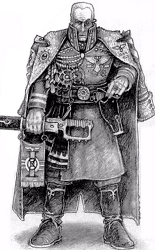
\includegraphics[width=\figwidth]{pics/14/3.png}
	\end{center}
\end{wrapfigure}
The Captain made a sour face. 
"It's not right for us to have to pay out of our own budget when we're operating openly like this. 
The Administratum's entire bloody purpose is to furnish us with whatever supplies we need." he grumbled. 
Sarge just stared at the ex-navy officer until the man leaned back in his chair and assumed a more businesslike tone. 
"Assuming FAIR market value," the Captain paused and shot a glare at the Quartermaster, who winced, "we picked up enough cargo during our tour of the border worlds to cover everything we need."

"Good." said Sarge, and turned to the Xenologist Adept. 
"That just leaves the more exotic parts Tink and Fio say they need for the Cells, which you've assured me will NOT be in stock, ESPECIALLY if it's the Inquisition asking."

The Xenologist held the dataslate up between himself and Sarge like a shield. 
"The only reason that some of the things on this list aren't class five forbidden xeno-tech, is because the Mechanicus has formally denied their existence."

Sarge rubbed his aching head. 
"Thank you for that reminder, but we really do need those parts. 
Luckily, Nubby says-" he paused as everyone in the room groaned, then started again. 
"Nubby says he Knows A Guy. 
So he, Tink, and Aimy are going to go do some trading of their own."

The Quartermaster hesitantly raised his hand. 
"Trading what?"
	
"I don't know, and I don't want to know." replied Sarge stoically. 
"So long as he gets the stuff we need, and doesn't start a shooting war with the local underworld or get arrested again, I'll be happy."

"That'll be a first." muttered the Captain, Sarge ignored him.

"Finally, Doc and Sister Valerie will be taking Gravis and any other critical patients to the Station's Medbay." Sarge turned to face the blank com-terminal and raised his voice. 
"Everything all ready to go Doc?" He was answered by a series of clanging crashes and a few indistinct curses.
\begin{wrapfigure}{O}{\figwidth}
	\begin{center}
		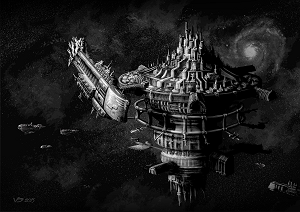
\includegraphics[width=\figwidth]{pics/14/4.png}
	\end{center}
\end{wrapfigure}
Sarge tensed at the sounds of mayhem coming through the comm, then relaxed as the crashes ended in a slamming door and a distant, but all-to-familiar, cackling laugh. 
He shook his head wearily, and leaned on the terminal's call button until the curses resolved themselves into Doc's rather harried voice. 


"I'm here, damnit! 
Everything is fine, Gravis is all ready to go, and the rest of the patients are stable enough to be left here for a few hours."

Sarge began to reply, but was cut off as the Captain interrupted him. 
"What about my Navigator, and your Psyker for that matter? 
Seemed like the bug really did a number on them."

"The Navigator woke up half an hour ago and scampered off back to his sanctum. 
Said he'd prefer to treat his own injuries." Replied Doc, raising his voice a little. 
Sarge barely made out someone in the background muttering about the "ungrateful damned mutant," but didn't comment on it as Doc continued. 
"As for Fumbles, I got his scrapes and bruises patched up, but I'm not sure if he suffered any mental damage from whatever the Zoanthrope did. 
I'd like to have the locals take a look at him, but Nubby… sprang him."

Sarge sighed. 
"Right, I'll have a chat with him after this." He closed the comm connection, and dialed in a new contact code. 
While the terminal chimed, he turned back to the rest of the room. 
"I think that covers everything, so if there aren't any questions," the Quartermaster began to raise his hand, but the Captain pulled it back down, "then we'll all meet in Bay 38A in..." Sarge faced the terminal as the channel opened, "ETA Bill?"

"Almost got the docking sorted, it’ll be about twenty-" there was a horrible crunching sound, and somewhere in the background a pressurization alarm started to wail, "ehh, call it forty minutes."

\greentext{>The All Guardsmen Party: Tyranid Delivery Experts}


\begin{wrapfigure}{O}{\figwidth}
	\begin{center}
		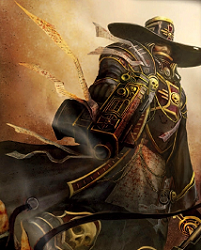
\includegraphics[width=\figwidth]{pics/14/5.png}
	\end{center}
\end{wrapfigure}
So no shit, there we were in Bay 38A, getting ready for our supply run, when Sarge walked in wearing the Evil Goon Uniform Alfred had fitted him with so long ago, a floor-length coat covered with skulls and buckles, and one of those stupid “Look at me I’m in the Inquisition” hats. 
We all froze for a few seconds, then Tink snickered, which was enough to set to rest of us off. 
We laughed ourselves sick while Sarge stood there and glared at us, I mean what else could we do? 
It was the most ridiculous thing we’d ever seen: 
he looked like a complete and utter pillock, and you could tell from his expression that he knew it too, the poor bastard. 
Hell, even the old Diplomat was laughing, and he'd been the one who'd forced Sarge to put the costume on.

Eventually Sarge got tired of just standing there while we laughed, and stalked over to where Nubby was rolling on the floor. 
After a few kicks and a little shaking had calmed the diminutive trooper down, there was a short discussion in which Nubby explained that Fumbles didn’t need medical attention: 
he just “ad a lil warpy ‘angover” which Nubby had taken care of himself. 
Sarge reminded Nubby what would happened if he’d given the psyker Narcotics again, and the greasy little trooper hastily explained that he’d just given Fumbles a few “tingies” of Guard-strong Recaff (you know, the sort you eat with a spoon, because it can't really be poured) and sent the psyker off to have a lie-down while the stuff kicked in. 
Upon further inquiry, it was revealed that "tingies" did not mean spoon-fulls or cups, and that Fumbles' resting place was one of the large crates on Nubby's team's cargo-pallet. 
Sarge guessed it was the crate that was vibrating.

\begin{wrapfigure}{O}{\figwidth}
	\begin{center}
		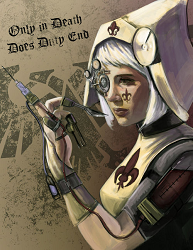
\includegraphics[width=\figwidth]{pics/14/6.png}
	\end{center}
\end{wrapfigure}
It took a lot of wheedling from Nubby, Tink, and even Aimy, but eventually Sarge accepted that Fumbles was somehow critical to their shopping expedition. 
And when I say "somehow critical," I mean that not even Nubby knew what he wanted the psyker for: 
when pressed he just shrugged and muttered about "genral in-su-rance." Anyway, Sarge accepted, mostly because Aimy was going along to make sure no one did anything overly retarded. 
When Doc arrived, and finished laughing, Sarge negotiated a temporary truce between him and Nubby in exchange for a promise to bring Fumbles to the Station's medbay as soon as he'd finished doing... 
whatever.

Speaking of Doc, he and Sister Valerie had an entire little medical convoy set up in the cargobay, waiting for the door to open. 
The whole array of kludged-together medical machinery keeping Sergeant Gravis alive had been put on wheels and strapped into something that looked like a sort of heretical mobile-torture device. 
It was bloody massive: 
between the air-tight freezer case containing the Space Marine's lower-half, the various crates full of his gear and the medical supplies they might need during the short trip, and the generator which kept everything powered, the whole thing weighed more than some tanks. 
It took three cargo servitors just to push it, and a pair of Valerie's minions to keep everything running while she sat there and handled each new medical emergency the Tyranid bio-weapon threw at her. 


After Doc had wandered back over to his girlfriend, Tink pointed out that, really, the medic should've been thanking them for keeping Fumbles away from that huge pile of delicate machinery. 
Everyone else quietly agreed.

\begin{wrapfigure}{O}{\figwidth}
	\begin{center}
		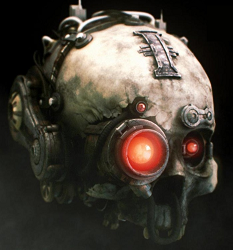
\includegraphics[width=\figwidth]{pics/14/7.png}
	\end{center}
\end{wrapfigure}
Now a clever observer, or at least one capable of counting to six, might wonder where Twitch was in this frenzy of preparation; 
especially since his relentless paranoia was half the reason that we were putting combat-mission levels of prep into a simple shopping trip. 
To put it simply, the demolitions trooper hadn't been invited aboard the station, and was holed up in a closet. 
This wasn't because he'd been having one of his moments and had threatened to destroy the entire station before whatever horrors it held devoured us all, at least not entirely. 
It was because we decided that we'd be damned if we were going to leave that bug unsupervised, and then come back to find out that it'd escaped, or been stolen, or turned into a reality-devouring portal to the warp. 


Since Sarge still held that leaving our semi-captive Tau scientist in charge of our other xenos prisoner was a horrendously stupid idea, and Twitch was the only member of the squad that didn't have a critical role in the shopping trip, he'd been put on guard duty. 
Twitch being Twitch, he'd accepted his mission, but decided that Sarge's orders to just sit in the Cells and watch the Zoanthrope were inadequate: 
they left the rest of the ship exposed to infiltration.

Initially Twitch had ran around the ship putting trip-mines on every airlock he could find, but that led to a rather heated argument with Hannah. 
Eventually, with Jim's help as a mediator, a compromise was reached, and Twitch traded his mines for fifty servo-skulls with detpacks strapped to them. 
Of course, the one problem with this arrangement, aside from the obvious, was that Twitch lacked any way to control the skulls. 
Luckily, he knew someone who could, and probably had nothing better to do.

So that's why Twitch, covered with detonators, was perched on a stool in a small, dark, cogitator-filled room, looking over the shoulder of our increasingly-nervous Cogitator Adept, as an army of suicide-skulls patrolled the ship.

\begin{wrapfigure}{O}{\figwidth}
	\begin{center}
		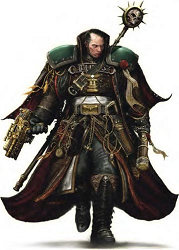
\includegraphics[width=\figwidth]{pics/14/8.png}
	\end{center}
\end{wrapfigure}
The Occurrence Border managed to dock with the station a mere three hours after the first attempt, which was a new record according to Ol' Bill, and the bay doors creaked open to revealed a rather angry-looking welcoming party. 
The pale Scribe and slightly-singed Techpriest at the head of the party looked around the bay for a few seconds, probably boggling at its bizarre layout or all the exposed wiring, then demanded to see the "Captain of this so-called vessel." Sarge stepped forward, his Inquisitorial costume flapping dramatically in the slight breeze caused by the various leaks in the bay's void-seal, and flanked by the Diplomat and Jim. 
The Scribe couldn't actually get paler, but he did turn a faint shade of green at seeing Sarge and hastily began apologizing.

The discussion that followed was highly amusing for us, both because the Scribe was terrified out of his mind, and because Sarge just stood there and looked stuffed. 
After he waved the Diplomat and Jim forward, he spent the whole time doing an impression of an especially grumpy exhibit in a wax museum. 
The only member of the welcoming party that wasn't unnerved by this was the damaged techpriest, but Jim chirped something in binary at his fellow cogboy, and the priest wandered off without saying a word. 
Between his terror and the fact that his only ally had just abandoned him, the Scribe was putty in our Diplomacy Adept's hands. 
All the little fees and fines concerning our docking were waved, the Station Security troopers were dismissed, and after one look at Sergeant Gravis, Doc's medical convoy was rushed off to the Station's main medbay.

Sarge, Jim, and the Diplomat were led out of the bay by the Scribe, bypassing the scanner-filled checkpoint that separated the docking bay from the rest of the station. 
The rest of us followed a conspicuously-slow Security guard to a side-door, which he sort of accidentally held open while picking up a bag of money that must've fallen out of his pocket.

\begin{wrapfigure}{O}{\figwidth}
	\begin{center}
		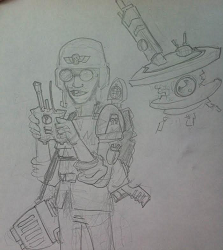
\includegraphics[width=\figwidth]{pics/14/9.png}
	\end{center}
\end{wrapfigure}
Our various trips through the Station went smoothly, for the most part, but left us all feeling a little nervous.

Sarge's group was led towards the Telepathica's headquarters by the nervous scribe along the Station's main corridors, and since the Diplomat was handling all the tedious smalltalk, he devoted his attention to scanning his surroundings. 
He didn't spot any overt threats, but there seemed to be more more Security officers around than were necessary, and it was obvious that the crowds around him were agitated about something. 
The most worrying thing he noticed was that his Inquisitorial costume didn't seem to be inspiring as much terrified silence as one would expect, instead it seemed to be causing a wave of excited chatter, and he could've sworn someone actually yelled "Woo! 
Inquisition!", which was worrying to say the least.

Those of us escorting the pallet of totally-not-contraband drew a lot less attention than Sarge. 
The corridors we'd been directed down by the corrupt security guard were occupied by the usual mix of laborers, drunken voidsmen on leave, and assorted scum that you'll find on any trading station. 
Between our insignia-less carapace armor, slightly-holey anti-scan cloaks, and the pallet of unlabeled crates, we fit right in. 


Nubby led the way, consulting a dataslate with directions to reach the Guy whom he Knew, while Aimy rather-grumpily pushed the pallet, and Tink lounged on Fumbles' box and played with his drone controller. 
The techie had de-skulled and stealthed Spot 2.0 at the first opportunity, and was happily inspecting the Station's infrastructure using the drone's sophisticated scanners and, occasionally, its cutting tools. 
Aimy ignored his wanton destruction of Station-property in the name of SCIENCE, but thumped him when he started ramming servo-skulls out of the air for kicks. 
Fumbles just sat in his box, radiating jittery excitement and hoping there was going to be a bathroom break soon.

\begin{wrapfigure}{O}{\figwidth}
	\begin{center}
		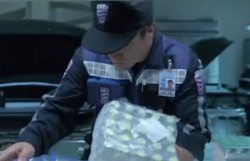
\includegraphics[width=\figwidth]{pics/14/10.png}
	\end{center}
\end{wrapfigure}
Down in the bowels of the station we noticed the same agitated atmosphere as Sarge noticed above, except with less Station Security and more burly mercs walking the street. 
Not being constrained by a need to appear all Inquisitorial, we pulled ourselves out of traffic and just began asking random people what was up. 
We quickly determined that either: 
a daemon-filled space-hulk had entered the system, a hive fleet was about to attack, all the astropaths in the Telepathica had been possessed by daemons, the Emperor's divine judgement for something or other was imminent, or random drunks and dockworkers were a terrible source of information. 
The closest thing to useful information we got was from a bored merc, who said that the "Pathica called a meeting of the Big Three" and advised Nubby to bugger off before he got a boot up the ass.

No one thought much of this information when we commend it to the rest of the team, except for Twitch, who got far too excited when he heard all the doomsday predictions, and Doc. 
The medic had arrived at the Station's Medbay without incident, but said he wasn't surprised the the Astra Telepathica had called a meeting, since the Medbay was absolutely packed with astropaths. 
He'd actually been told by the head medicae that Sergeant Gravis would have to wait his turn, and they'd been shuffled off into a storage bay since no real rooms were free. 
Sister Valerie was not pleased with this treatment, but Doc was looking on the bright side, and began looting antidotes and other medical supplies with the sort of enthusiasm one would usually expect from Nubby.

Since a whole pile of injured Astropaths is generally considered to be a bad sign when visiting a space station, Sarge made slightly-grumpier faces at the old Diplomat until he got the hint and started asking the Scribe pointed, but still very diplomatic, questions. 
Unfortunately, the Scribe just fell back on the Chain of Command, and promised his boss would fill us in.

\begin{wrapfigure}{O}{\figwidth}
	\begin{center}
		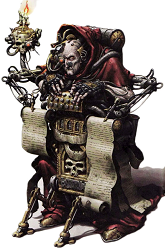
\includegraphics[width=\figwidth]{pics/14/11.png}
	\end{center}
\end{wrapfigure}
When Sarge entered the headquarters of the local branch of the Astra Telepathica, the first thing he noticed was the blood. 
In his professional opinion, the density and pattern were more akin to a what you'd find in a field aid station as opposed to an ambush site. 
This was not a very useful observation, but he still felt rather proud: 
it was definitely the sort of thing an Inquisitorial agent was supposed to notice. 
The Scribe led Sarge and his team through the bloody lobby, down some slightly-less-gory hallways, and finally to a blood-free meeting room occupied by what Sarge initially assumed was a transcription servitor. 
Sarge barely managed to hide his shock when the pile of augmetics, paper, and data feeds lumbered upright and introduced himself as the Prefect of the local division of the Adeptus Administratum.

The Diplomacy Adept did his thing, introducing Sarge and Jim, and expressing surprise that we were meeting the head of the local Administratum as opposed to someone from the Telepathica. 
The Prefect wheezily explained that the Choir-Master was currently indisposed, but had called a meeting to discuss the "incident", and would arrive, along with the President of the Shipmasters' Union, as soon he was able. 
There was a lot of diplo-speak about how glad the Prefectus was that Sarge would be able to participate in the meeting and how in the meantime he'd be able to assist us with anything we needed for our own mission. 
The whole group, nervous Telepathica Scribe included, filed off into a small attached suite and began going through the list of parts and services we needed. 
Sarge allowed himself a brief moment of hope that we'd be able to get everything we need before getting bogged down in whatever the locals' problem was, then just leave if it looked too hairy.

Poor, optimistic Sarge.

\begin{wrapfigure}{O}{\figwidth}
	\begin{center}
		
\includegraphics[width=\figwidth]{pics/14/12.png}
	\end{center}
\end{wrapfigure}
Getting official approval for Sergeant Gravis' medical treatment was easy, and the Prefect seemed confident in the local Medicae's ability to fully treat Tyranid bio-weapon that'd infected him. 
Likewise, most of the stuff on Jim's part list was accepted without comment. 
The first hiccup was when we got to some of the really powerful psi-resistant materials: 
the Prefect claimed they were in stock, but couldn't be released without authorization from the sub-sector capital or the official use of an Inquisitorial seal. 
He claimed that due to the "incident", it would be a long and difficult process to get authorization, but he saw no other option if we wanted to be discreet. 
Sarge pondered this for all of three seconds, decided discretion was overrated anyway, pulled out his Interrogator's Rosette, and plugged it into a proffered dataslate.

The Prefect seemed quite happy that everything was going to be above-board for once, saying that after the code was verified by the Telepathica's databases, there'd be no trouble getting the materials or anything else on the list. 
Sarge cheered up at this, and was considering asking to add the fuel bill to the list, when the Prefect added "except for the Astropathic messages." With that, the discussion finally turned to the "incident".

According the Prefect, roughly half a day ago some sort of psychic attack had hit the station. 
Every Astropath who had been working in the Choir-Chambers had suffered a severe case of exploding-head, and those who hadn't been on-duty had suffered everything from nosebleeds, to seizures, to complete mental breakdowns. 
It wasn't just limited to the Astropaths of the Telepathica either, several of the ships in system had lost their astropaths, and other varieties of sanctioned psykers had been affected too, albeit to a lesser degree.

\begin{wrapfigure}{O}{\figwidth}
	\begin{center}
		
\includegraphics[width=\figwidth]{pics/14/13.png}
	\end{center}
\end{wrapfigure}
At a wave from the Prefect, the Telepathica Scribe, who'd been doing his best to avoid the attention of the big scary Inquisition people, spoke up. 
He said that some of the more lucid Astropaths had started piecing together details about the psychic attack. 
It had originated in the outer system and had probably come from a ship heading to or from the station. 
The popular theory was that some terminally greedy Rogue Trader was hauling a heretical artifact, or massively powerful psyker, or possibly even a bound daemon into the Imperium to sell to a cult or something, and it'd lashed out at the large concentration of psykers on Station for some reason.

It was at this point that Sarge began to feel really uneasy. 
Not because he suspected that there was a Daemon or heretical Rogue Trader running around the system, but because he suspected there wasn't. 
With a rising sense of dread, our heroic leader asked the Scribe if any of the surviving astropaths had been able to describe what the attack had felt like. 
When he heard the words "a million barbed legs ripping across their minds" Sarge's composure cracked. 
He leaned back, covered his face with his hands, and quietly cursed to himself until the Prefect asked what the problem was. 
In fit of retardation, Interrogator Greg Sargent answered him truthfully.

The silence that filled the room when Sarge told the two Stationers that it had been OUR cargo that'd killed half the Astropaths in the system was incredibly unpleasant. 
The weary apology that Jim added after a few minutes just made it worse. 


Eventually the horrible silence was broken by the sound of the Prefect's augmetics going *DING* and spitting out a long strip of paper. 
Sarge caught a glimpse of it and thought it looked liked a sort of receipt or budget report, and the last number had a lot of digits. 
The Prefect reviewed the paper for a few seconds, then tucked it away, hauled himself upright, and said he'd return after the search had been called off.

\begin{wrapfigure}{O}{\figwidth}
	\begin{center}
		
\includegraphics[width=\figwidth]{pics/14/14.png}
	\end{center}
\end{wrapfigure}
As the Prefect left, he handed the dataslate Sarge had plugged his rosette into to the transfixed Scribe. 
He told the flunky to go run the code, THEN go fetch Choir-Master. 
Hopefully the knowledge that the whole thing was going to be an Official Inquisitorial incident instead of a cloak and dagger charade would keep the man calm. 
When the two Stationers had left the suite, the old Diplomacy Adept pulled out a small device which emitted a sort of low buzzing sound, and rounded on Sarge and Jim.

The lecture Sarge and Jim got was scathing and brought back painful childhood memories involving unfinished homework assignments and failed tests. 
It started with the importance of never admitting fault and maintaining at least the appearance of competence, and then shifted into a general lecture on how to react to a diplomatic crisis. 
Sarge bore the lecture stoically, automatically standing at attention and adopting the blank expression employed by NCOs across the galaxy. 
His only movement during the whole thing was to put his combead on mute when the rest of us figured out what was going on and started snickering. 
Jim just turned his ears off after the first minute.

After what felt to Sarge like half a millennium, the old Diplomat's lecture concluded with a bitter comment about how, on top of everything else, the Scribe had run into the Choir-Master on his way to verify our identity. 
Sarge blinked as the Diplomat detailed how the head Astropath was too angry to even form coherent sentences, and had either punched a hole through a wall or severely broken his hand. 
After a thoughtful pause, Sarge asked the Adept how exactly he knew this, and got a pithy reply about diplomacy being as much about listening as talking.

\begin{wrapfigure}{O}{\figwidth}
	\begin{center}
		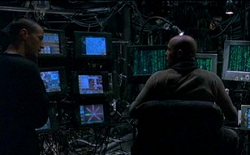
\includegraphics[width=\figwidth]{pics/14/15.png}
	\end{center}
\end{wrapfigure}
It took Sarge and Jim a little while to figure out what was going on, mostly because Jim had to be brought back up to speed after he'd turned his hearing back on, but they worked it out eventually. 
The old Diplomacy Adept admitted that he'd placed bugs on both the Scribe and the Prefect. 
Also, he'd planted a few discrete data uplinks too, so assuming our Cogitor Adept hadn't been driven to complete distraction by Twitch, we probably had access to all unencrypted comm traffic on the station.

It turned out that he was correct: 
when asked, the Cogitator Adept said he had the network cracked completely open. 
Additionally, he'd be able to get into the security cameras if someone could PLEASE convince Twitch to just sit down and watch the skulls' feeds instead of badgering him about changing their patrol routes every ten seconds. 
Sarge, who was somewhat grumpy about not being informed of all the spy stuff beforehand, told Twitch to Sit Down and Shut Up, and demanded to be kept up to date on what the Prefect and Choir-Master were doing.

So Sarge sat there listening to reports. 
Learning that the Choir-Master had taken the Scribe's dataslate and had gone off to verifying our Inquisitorial credentials personally, and the Prefect was still in the process of standing down the Station's defenders with the aid of the recently arrived President of the Shipmasters' Union. 
Meanwhile, Doc had finished looting everything of value from the storage bay that Gravis' had been shuffled into, and had taken over the Space Marine's treatment while Sister Valerie went to "have a word" with the Station's head Medicae about how long the wait had been. 
Doc made her promise not to start a fight, or refer to the wounded Astropaths as "warp-tainted mutants".

\begin{wrapfigure}{O}{\figwidth}
	\begin{center}
		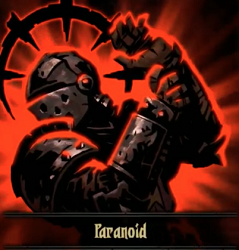
\includegraphics[width=\figwidth]{pics/14/16.png}
	\end{center}
\end{wrapfigure}
Back on the Occurrence Border, Twitch had grumpily followed Sarge's order and was watching as the Cogitator Adept began pulling in vid feeds from the Station. 
Soon every screen in the room was filled, either by a feed from the Station, or one from the suicide skulls, and for a brief moment Twitch felt like he'd become a god, between the vid feeds from the Station and the ones from his suicide skulls, he could see EVERYTHING. 


Twitch could see the corridors around the dock, some of them filled with busy people, others sealed and empty. 
He could see crewmen hauling goods in and out of the docking bay, and the Captain arguing over price with a harassed-looking Stationer. 
He could see Fio working diligently in the Psyker Holding Cells and trying to ignore the way the Zoanthrope's metal-plated face seemed to follow him despite the stasis field. 
He could even see Nubby, Tink, and Aimy as they checked various seedy bars for their black market contact. 
For the first time in years, Twitch's paranoia faded away as it was replaced by an overwhelming feeling of Control.

It lasted all of fifteen seconds, and then something inside the jumble of warped and twisted mental gears that made up Twitch's mind went *PING*. 
Twitch reeled as his mind automatically began cataloguing every single suspicious object, which is to say every man, woman, child, animal, servitor, and overlarge barrel on the Station. 
He wound up sprinting from the room, leaving the confused, but relieved, Cogitator Adept to monitor everything in peace, while he went to go put as many explosives as possible between himself and the horrible mass of potential threats that was the Station's population.

A few minutes later, the rest of us were informed by the Cogitator Adept that Twitch had begun booby trapping every locked door, air vent, and maintenance hatch in the docking bay. 
We decided that, all in all, it was better just to let him do it, and warn the Stationers to only use the main entrance.

\begin{wrapfigure}{O}{\figwidth}
	\begin{center}
		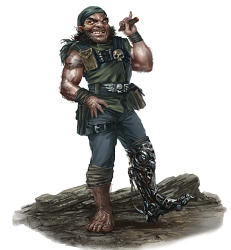
\includegraphics[width=\figwidth]{pics/14/17.png}
	\end{center}
\end{wrapfigure}
While Twitch, Doc, and Sarge did their respective things, the rest of us finally reached the last stop on our tour of just about every shitty bar in the Station. 
Thankfully, despite how long it'd taken to figure out which venue was "the place with the curly thing on its sign, y'know the one across from the food place that serves the stuff with the sauce" the search had gone relatively smoothly. 


"Smoothly" in this case meaning that: 
no one asked to inspect our boxes, Nubby was never CAUGHT with his hand in someone's pocket, Tink kept his mouth shut the whole time and didn't trip any alarms while poking around with his drone, nobody saw Fumbles when we let him out to use the bathroom, or found out that what happened to said bathroom had anything to do with us, and Aimy only lightly-pummeled the bouncer who'd referred to her as "sister", and later admitted that the man probably hadn't meant it as a comment about her hair.

We found the Guy Who Nubby Knew at the back of the bar, sitting on an extra-high stool. 
Aimy, who was a Markswoman after all, didn't even blink at the realization our black market contact was a Ratling, but Tink did a doubletake. 
As Nubby sidled up to the miniscule marketeer, Tink eyed the pair and asked, with his usual lack of tact, if there was some sort of height limit on being a thieving bastard. 
Thankfully, the half-dozen other Ratlings in the bar were too focused on Nubby to notice the comment. 
Aimy told Tink to stick with the pallet and try to keep his mouth shut, and watched as Nubby "did 'is fing".

\begin{wrapfigure}{O}{\figwidth}
	\begin{center}
		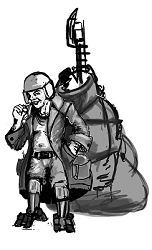
\includegraphics[width=\figwidth]{pics/14/18.png}
	\end{center}
\end{wrapfigure}
Now, Nubby's heritage had been a matter of much speculation back in the Guard. 
Not in the sense of who his parents were, because even he admitted figuring that out was a lost cause, but as to what horrible combination of Human, Abhuman, Farm Animal, and possibly Gretchin genetics had produced such a "unique" individual. 
Determining what to put the trooper's species down as had been a trial for several munitorum clerks, and eventually the issue had to be sorted out by the Commissar. 
He'd decided that, for lack of any better fit, and because the Generian 99th was not officially a mixed-species unit, Nubby was Human. 
He'd even issued the disgusting little trooper an official card saying so, just to avoid the discussion coming up again.

The point is, that Nubby, much to the relief of the entire race, was NOT a Ratling. 
Despite (or possibly because of) this, Nubby had always gotten on very well with the little buggers, and this case was no exception. 
After a bit of amiable chatter, the Marketeer and a few of his half-pint bodyguards led us off to a discreet warehouse to talk business. 


At the door all of us, except for Nubby, who they were understandably reluctant to frisk, were subjected to a very thorough security check. 
Our anti-scan cloaks, knives, las-pistols, holdout weapons, and the home-made shockstick which Tink insisted on calling his "Power Wrench" were temporarily put aside, and we were each asked to supply a little bit of blood. 
They put the blood into some sort of scanner, which they claimed was checking to see if we were psykers, genestealers, polymorphine users, or anything else which might compromise the deal. 
We passed of course, and were allowed to keep our combeads, electronics, and even our weapons, since Nubby was a "known factor." Also, because the warehouse was monitored by a dozen remote controlled las-turrets.

\begin{wrapfigure}{O}{\figwidth}
	\begin{center}
		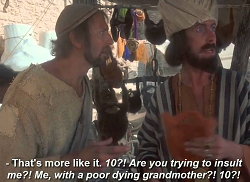
\includegraphics[width=\figwidth]{pics/14/19.png}
	\end{center}
\end{wrapfigure}
Once inside the black market warehouse, which looked exactly like a normal one, except for the large number of armed men in the front office and fact that every single crate was labelled excessively mundane things, we got down to business. 
At Nubby's signal, we started by opening a few of our crates of "recreational materials" and "military surplus", to convey that we were rather serious, and then handed over our shopping list. 
The change in the Marketeer's demeanor as he reached the more esoteric items on our list was remarkable. 
He went from stereotypical jovial Ratling to serious, and slightly nervous, businessman in seconds, and ordered his retinue and the warehouse's workers out. 
Once the room was clear, what had to be the most vicious bout of haggling in the history of the Imperium started.

Despite possessing the charisma, and odor, of a week-dead grox on a hot day, Nubby's deep familiarity with all aspects of criminality and his ability to wheedle, whine, importune, and blatantly lie had always served him well when it came to back-alley negotiations. 
The Ratling wasn't a slouch when it came to haggling either, and responded with an equal amount of cunning viciousness. 
Aimy and Tink were both taken aback by the ferocity of the argument, which seemed barely short of homicidal, but as it continued without either Nubby or the Marketeer trying to kill each other, the two troopers adjusted to the situation and even tried to lend Nubby a hand in his negotiations when they thought they understood his plan. 
They failed abysmally, of course.

Between their actually-insulting insults, miscalculated threats, and lack of knowledge as to how the value of goods changed after they'd fallen off the back of a shuttle, Aimy and Tink put such a dent in Nubby's progress that negotiations had to be temporarily paused. 


\begin{wrapfigure}{O}{\figwidth}
	\begin{center}
		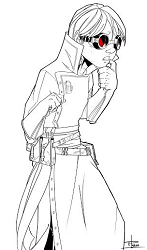
\includegraphics[width=\figwidth]{pics/14/20.png}
	\end{center}
\end{wrapfigure}
Once Tink and Aimy had been relegated to helping the sole cargo-servitor that had remained in the room fetch boxes, the haggling resumed. 
Crate after crate of narcotics, dubiously acquired valuables, and those well made and untraceable small-arms the Inquisition issues were exchanged for xenos-made circuits, tools, and materials.

At first it seemed like our supply of illicit goods was going to run short before we had everything on Tink and Fio's list, but as the negotiations continued, the Marketeer became more and more relaxed and generous with his exchanges. 
A careful observer might have noticed that the change in the Ratling's attitude seemed linked to how much time he spent within twenty meters of the cargo-pallet, and how Nubby, Aimy, and Tink tended to stay away from said pallet.

This was, of course, what Nubby had wanted Fumbles for. 
They'd pulled this sort of con quite a few times, though usually not with Fumbles was encased in a shipping crate and hopped up on a downright unhealthy amount of stimulants. 
The psyker wasn't directly messing with the Marketeer's mind, that'd be too obvious to any observers as well as the Marketeer himself when he walked out of range, and honestly we didn't trust Fumbles to do that sort of thing for any length of time without something exploding. 
Instead the little psyker was just sitting there, concentrating on thinking calm and happy thoughts, and letting his aura do the rest.

With Fumbles' help we made it down to the last item on our shopping list with two crates, not counting Fumbles' and our other backup crate, still unopened. 
Unfortunately, that last item was a sticking point: 
not even under the effects of the feel-good aura, and with a big box of only-slightly-warp-tainted Servitor Control Units up for offer, the Ratling refused to even admit he knew what Wraithbone was, much less part with a big ol' chunk of it. 


\begin{wrapfigure}{O}{\figwidth}
	\begin{center}
		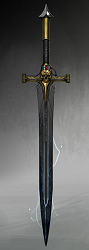
\includegraphics[width=\figwidth]{pics/14/21.png}
	\end{center}
\end{wrapfigure}
Nubby eyed Tink, who implied via gesture that we REALLY needed a piece of Wraithbone (despite the fact that he actually had no idea what Fio wanted it for). 
With a pained mutter about how he'd been intending to save it for his retirement, Nubby cracked open our last non-emergency crate. 
Aimy swore, Tink let out a jealous sigh, and the Marketeer's jaw dropped halfway to the floor as Nubby drew out a Mastercrafted Powersword larger than he was and bearing a crossed-scythe sigil on its crossguard. 
In the silence that followed, Nubby, teetering under the weight of the sword, asked the Ratling if he was SURE he didn't have any Wraithbone in stock.

Nearly a kilometer away, Sarge's NCO senses tingled, and he was seized by the feeling that something had just happened that he was going to be VERY angry about. 
He didn't have any time to dwell on this feeling though, because right then the Cogitator Adept commed to say that a huge amount of traffic had just hit the Station's net. 
He didn't mention what was actually being said though, and when Sarge asked, the Cogitator Adept responded with a bunch of techno-jargon, so Sarge told Jim to handle it and turned to the Diplomacy Adept, who'd gone all fidgety. 


When Sarge asked what the problem was, the old Diplomat revealed that the Choir-Master had finally re-entered the range of his bugs, and was absolutely enraged with the Prefect, as well as the Scribe and the President of the Shipmaster's Union. 
So far all the yelling had been about talking to us without him being present and other unilateral decisions, but the Adept was sure there was some other cause, and promised to keep Sarge up to date.

\begin{wrapfigure}{O}{\figwidth}
	\begin{center}
		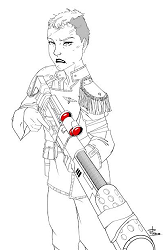
\includegraphics[width=\figwidth]{pics/14/22.png}
	\end{center}
\end{wrapfigure}
Back down in the warehouse, the miniature Marketeer had recovered from his shock and was inspecting the quality of the Powersword while Nubby chattered at him from just outside Fumbles' radius. 
Behind them, Aimy and Tink dug out the small crate labeled "Talc-10kg" the Ratling had directed them to, and complained at eachother. 
Aimy was in the middle of telling Tink, who was too busy whining about how much he'd wanted to dissasemble that sword to even pretended to listen, that Sarge was going to blame HER for this, when she noticed the Ratling freeze. 
After a quick kick to his shin, Tink noticed too, checked the screen of his drone controller, and gave Aimy a thumbs up. 


As Aimy and Tink came over to see what the problem was, Nubby finally realized that the Marketeer wasn't listening to his list of things he'd accept as "change" for Gravis' Powersword and the Control Units (y'know, since they were obviously worth WAY more than a spooky chunk of rock). 
He sidled up to the frozen Marketeer and tapped him on the shoulder. 
The Ratling spun around, still gripping the sword, and Nubby jumped back with a little scream as the movement triggered a VERY painful memory. 
This in turn set off the Ratling, who held the sword in front of him like a shield, and hastily began backing up and gibbering about needing to use the bathroom.

We all watched as our black-market contact ran out of the room and slammed the door behind him. 
Aimy let out a pained sigh, and asked Nubby if there was any chance the Ratling would be coming back, or could at least be convinced to return the Powersword before trying to kill us. 
Nubby just cackled, and began divvying out our big-boy guns from one of the remaining boxes, while Fumbles burst from the other, began shouting about how we were all going to die, and immediately faceplanted as his still-asleep legs betrayed him. 


Aimy caught her rifle and casually headshot the warehouse's cargo servitor, then sighed again and activated her combead.

\begin{wrapfigure}{O}{\figwidth}
	\begin{center}
		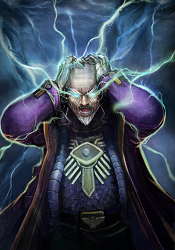
\includegraphics[width=\figwidth]{pics/14/23.png}
	\end{center}
\end{wrapfigure}
Sarge's response to the news that Nubby's black-market deal was about to turn into a shootout was nowhere near as sarcastic as Aimy had anticipated. 
This was because her report was interrupted by Jim and the Cogitator Adept discovering that the source of all the chatter on the Station's net was a MASSIVE bounty that'd just been placed on all crewmembers of the Occurrence Border by the Astra Telepathica. 
This worrying news was interrupted in turn by the Diplomacy Adept's report that the Choir-Master had just declared our Inquisitorial credentials to be completely falsified, and was in the process of convincing the others Station leaders to sic everything they had on us.

That last piece of bad news came as a surprise, because we knew that Sarge's Rosette was genuine, and there was no way it could have just malfunctioned either: 
Inquisitorial Rosettes and the Verification Databases are built to last. 
That meant this wasn't some sort of accident: 
the Choir Master had obviously come unhinged and was out for vengeance.

I mean it was sort of understandable, he'd just had his brain half-fried by a psychic blast which had also killed a whole bunch of the closest thing he had to a family, and the whole thing was technically our fault… Justifications aside though, after he ran our credentials he must have decided that he didn't like the answer, or he might not have even bothered checking at all, and now he was lying to the other Station leaders about how we were vile heretics impersonating Inquisition Agents. 
They believed him too, by the time we'd figured out via the bugs what was happening, he had the Prefect and the President completely convinced.

There was obviously no chance of talking the Stationers around, all Sarge and the Diplomat could do was sit there and listen as they argued about the best way to round all of us up and "bring us to justice". 
The situation was FUBAR, to say the least, and all this news hit Sarge at once.

\begin{wrapfigure}{O}{\figwidth}
	\begin{center}
		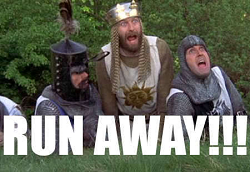
\includegraphics[width=\figwidth]{pics/14/24.png}
	\end{center}
\end{wrapfigure}
Now this is where some men might have gone into shock, or exploded in irrational anger, or sunk into despair, but not Sarge. 
He allowed himself half a second of ironic satisfaction at the way his cynicism had, once again, been justified, then removed that stupid Inquisitorial hat and started belting out orders. 
Admittedly, those orders were to just do what we would've done anyway, but as someone or other said, "Never give an order that won't be obeyed." 

So, as a reminder, we were split up into four groups. 
Well, five if you count the Captain, but when Sarge commed him to report the situation and coordinate things, the ex-navy Officer just told Sarge to do something anatomically improbable, and said he'd meet us back on the ship. 
Judging by the amount of gunfire and screaming in the background, he had things under control. 
Anyway, Doc was stuck in the Station Security-filled medbay in the mid-north part of the Station, Aimy and company were in a warehouse on the lower levels of the eastern side of the station, Twitch and the Occurrence Border were at the west-most docking bay, and Sarge was almost at the top of the central spire. 
 

Our options were limited, we were split up, ass-deep in increasingly hostile territory, and, in Sarge and Doc's cases, practically unarmed. 
We did have a ship-full of armsmen, plus a few nearly-functional lance batteries, but the Stationers knew that and were already deploying men in that direction. 
We were far too outnumbered, outgunned, and (though it pains me to admit it) ethical to start an all-out war. 
Plus, it's a bad idea to blow holes in a space station while you're still on it. 
They'd have to sit back and hold down the fort while we did our best impression of a bunch of Catachans on their way back to base after a night on the town.

It was time to fall back on that old Guard classic: 
Regroup, Retreat, Repeat.

\begin{wrapfigure}{O}{\figwidth}
	\begin{center}
		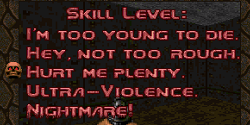
\includegraphics[width=\figwidth]{pics/14/25.png}
	\end{center}
\end{wrapfigure}
The plan, if you could call it that, called for Doc, who was exposed, surrounded, had no idea where Sister Valerie was, and still had his hands quite full with Gravis, to sit tight and hope that no one remembered which closet he'd been shuffled into. 
Aimy, Tink, Nubby, and Fumbles, would load up all the loot they could carry (as if they needed telling), make their way to the medbay to collect Doc, and then the whole group would head for the ship. 
While they traversed the station, Twitch, along with the suicide skulls and any armsmen he could find, would keep the locals out of the docking bay and the Occurrence Border. 


As an afterthought, Sarge asked Twitch to try to keep things as non-lethal as possible: 
on the off chance that we'd have an opportunity to try and smooth things out, it'd be nice not to have a four-digit body count to deal with. 
He may have given Aimy a similar order, but some freak comm-interference (which sounded a lot like Nubby and Fumbles blowing on their combeads) scrambled the message.

Everyone except Doc liked the plan, but it did have one problem: 
it didn't cover how Sarge would get out of the Astra Telepathica headquarters. 
We pointed this out, and were told to shut up, do our jobs, and let Sarge take care of himself. 
The rest of us interpreted this as a clear sign that Sarge had no idea what he was going to do, but since we didn't have any suggestions more useful than sarcastic comments about "handle it," we left him to it.

\begin{wrapfigure}{O}{\figwidth}
	\begin{center}
		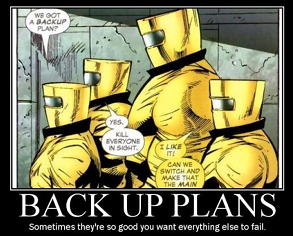
\includegraphics[width=\figwidth]{pics/14/26.png}
	\end{center}
\end{wrapfigure}
Once the rest of us had started moving, Sarge muted his combead, swore a lot, then took stock of the situation. 
He was in a small office and bathroom suite with only one exit, which lead to a large conference room. 
Said room was probably occupied by a few of the Choir Master's bodyguards, who would be watching to make sure he didn't go anywhere while the Station's leaders plotted their attack. 
His assets consisted of:

\greentext{>1 Laspistol (Standard Inquisition Issue)}

\greentext{>4 Laspistol Power Packs (Charged)}

\greentext{>1 Combat Knife (Notched)}

\greentext{>1 Roll of Duct Tape (Olive Green)}

\greentext{>1 Combead (Muted)}

\greentext{>1 Inquisitorial Costume, with Hat (Stupid)}

\greentext{>1 Three Hundred Year Old, Bug-Planting Diplomat (Grumpy)}

\greentext{>1 Jim (Whimpering in a Corner About How Everything Keeps Happening to Him)}


This was not, of course, anywhere near enough to take on the small army of armsmen, gun servitors, and very-angry psykers inhabiting the Astra Telepathica, not to mention the Station Security forces outside. 
In fact, by Sarge's reckoning, it probably wasn't even enough to take the six to eight body-guards that the Choir Master had brought with him, but the Diplomacy Adept disagreed. 
The aging Diplomat drew an ornate las-pistol from his robes, and suggested taking the Station's leadership hostage while they were still only a few rooms away. 
When Sarge just stared at him, he explained that with sufficient "leverage" it'd be easy to re-open negotiations and smooth everything over. 
After a few more seconds of staring, Sarge decided that nothing the old Diplomat did or said would surprise him anymore, and made "Fight through a bunch of heavily armed men and start a volatile hostage situation" Plan B.

\begin{wrapfigure}{O}{\figwidth}
	\begin{center}
		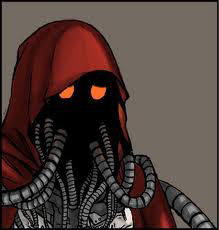
\includegraphics[width=\figwidth]{pics/14/27.png}
	\end{center}
\end{wrapfigure}
In a desperate attempt to come up with a Plan A, Sarge reactivated his combead and asked the Cogitator Adept to try to find the spire's blueprints, and then began checking if the suite's air vents were large enough to crawl through. 
Jim, who was huddled in morose little ball, told Sarge not to bother: 
it would be incredibly stupid to make air vents large enough to fit a person. 
Sarge tried to defend his idea by pointing out that the Occurrence Border was littered with such vents, but Jim patiently explained that this was only because the Occurrence Border was an incredibly stupid ship. 


Sarge relented, but in the silence that followed, the Cogitator Adept pointed out that there were a few maintenance shafts on the Telepathica's blueprints that could be crawled though, if Sarge could open them that is. 
Jim attempted to shoot this idea down as well, explaining that such shafts would be heavily monitored by the local Mechanicus, who'd report our movements to the Station government. 
Sarge had grown rather cross with Jim by this point, and angrily told the Enginseer to either DO SOMETHING about that, or help think up a better idea.

Jim went quiet at that, then got really thoughtful look, and went over and jacked himself into the suite's comm terminal. 
He didn't respond when asked what he was doing, so Sarge assumed it was something important, and decided to focus on keeping the suite secure until Jim finished whatever it was.

\begin{wrapfigure}{O}{\figwidth}
	\begin{center}
		
\includegraphics[width=\figwidth]{pics/14/28.png}
	\end{center}
\end{wrapfigure}
Way down in the black market warehouse, Aimy and Tink put the finishing touches on the cargo pallet. 
Said pallet looked nothing like the one that had left the Occurrence Border: 
for one thing it was much fuller than it used to be, the stack of crates on it was nearly three meters tall, and they were held in place by dozens of straps and tarps. 
Because this was far more weight than the pallet could handle, or anyone wanted to push around, a few grav-plates had been scrounged from the warehouse by Nubby, and more or less randomly slapped on. 
Finally, the treaded bottom half the warehouse's cargo servitor had been fastened on as an incredibly grisly external motor. 
The thing looked horrible, with a coat of red paint and a few stubbers you could pass it off as an Ork Trakk, but it handled surprisingly well.

The only interruption during the whole loading and modification process had been about a minute after the Marketeer had fled, when the las-turrets in the ceiling had suddenly swiveled to track us, and then went still as the EMP grenades Spot 2.0 had placed on them went off. 
There'd been no other attempts to kill us, partially because Tink had used his heavily-modified plasma gun to weld the warehouse's doors shut, but mostly because of Fumbles. 
The hyped up psyker spent the whole time jittering back in forth in front of the main entrance, emanating all sorts of mental unpleasantness at anyone who got near it. 
He claimed that after the third time the Ratlings had lost their nerve, they'd decided that, since they had all the warehouse's exits covered, they could spare the time to call in a few teams of disposable bigguns to tackle the scary guardsmen for them. 
The major flaw in their plan was that we had the aforementioned heavily-modified plasma gun, and no intention of leaving via the doors.

\begin{wrapfigure}{O}{\figwidth}
	\begin{center}
		
\includegraphics[width=\figwidth]{pics/14/29.png}
	\end{center}
\end{wrapfigure}
After a quick call to the Cogitator adept to pinpoint a hallway below us, Tink set his plasma gun to cut, and added an exit ramp to the black market warehouse. 
He did a very good job of it too, managing to pick a section that didn't have any water or sewage pipes and was long enough for the ramp to come down a nice, gentle twenty degrees. 
Honestly Tink did such a good job that the Ratlings should have paid us for adding the exit ramp, it was real professional work, and we made sure to point that out in the note.

We left a note for the Marketeer because, honestly, we felt a little bad about how things had turned out. 
We really hadn't intended to rip off the anyone. 
I mean sure, we'd snuck in a psyker, a stealth drone, and enough weapons to kill anyone who argued with us, but that was just reasonable precautions. 
We'd had every intention of playing things straight with them… or at least only moderately crooked. 
The point is, we understood that their attempt to betray us was because of the whole Telepathica thing, not something personal, and Nubby really wanted to keep doing buisness with them after this was all cleared up.

So while Tink worked, Nubby put together a little note explaining how there were no hard feelings, and that we were only taking a reasonable "seveny-free percen: 
trying ta kill us pen-all-tee". 
It should be noted that this rather precise percentage wasn't some arcane black-market custom, it was just the amount of stuff we were able to fit onto the pallet. 
Anyway, the penalty took the form a few of the things that Jim had been intending to get from the Administratum, plus a few of our own crates. 
At Aimy's insistence, these did not include the damned, literally in this case, Servitor Control Units or any of the other stuff Nubby had kept in the Cogtain-crater room. 
Those could be someone else's problem.

When Tink was finished, we taped the note to what was left of the cargo-servitor, gathered up Fumbles and got the hell out of there.

\begin{wrapfigure}{O}{\figwidth}
	\begin{center}
		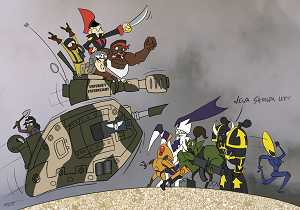
\includegraphics[width=\figwidth]{pics/14/30.png}
	\end{center}
\end{wrapfigure}
Our trip through the station was shockingly swift, stealthy, and professional. 
At least for certain values of "stealthy" and "professional", but there's no debating the "swift" part, or the "shocking" for that matter. 
Since our dismembered-servitor propulsion system was capable of pushing the loot pallet at speeds best described as "unsafe", we piled onto it and sped through the corridors like… Well, like a bunch of drunken guardsmen on leave.

Thanks to the maps provided by the Cogitator Adept, the scouting abilities of Spot the Wonder Drone, and a plasma-gun-enabled disregard for inconveniently placed doors and walls, we took a very direct and underpopulated route to the medbay. 
That's not to say that we didn't run into anyone on our trip, but thanks to Spot and Fumbles, we generally saw them before they saw us. 


We managed to avoid or sneak by a few potential witnesses, as well as some Mercs and Security officers. 
Others were handled by sucker-punches and the application of Tink's not-actually-a-power-weapon Power Wrench. 
When that wasn't an option, we had Fumbles cloak us, or edit a few memories, though sometimes this didn't work either, and a more efficient approach was called for. 
Violence was only our last resort mind you, it's not like we were some sort of high speed murder-barge shooting down the Station's corridors with no regard for collateral damage, innocent lives, or speed limits. 
At least not most of the time.

Anyway, if you disregard maimings, psychic trauma, property damage, and other little things like that, our expedition was practically bloodless. 
Which is to say that there were DEFINITELY under 10 deaths, and most of those were Mercs and Bounty Hunters, and everyone knows they don't really count. 
Oh, and the maintenance worker that got ran over by the loot-pallet really should've known to look both ways before entering such a long and obstruction-free corridor, and had probably been drunk anyway.

\begin{wrapfigure}{O}{\figwidth}
	\begin{center}
		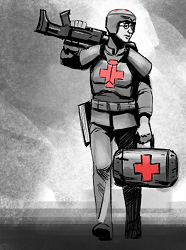
\includegraphics[width=\figwidth]{pics/14/31.png}
	\end{center}
\end{wrapfigure}
Despite the incredible speed of the loot-pallet, we reached the medbay considerably behind Station Security. 
This was hardly surprising though: 
they'd had several teams guarding the place since it was currently home to half the Station's surviving Astropaths. 
Luckily, Doc was a big boy who could look after himself, and he had kept the rest of us up to date on his situation while we travelled.

Doc's initial situation had been about as bad as Sarge's: 
the Stationers knew he was in the medbay, he had nothing but his sidearm, and there was no way he could get Gravis out without being noticed. 
Some of us had suggested leaving the torso-fied Space Marine behind and hoping the Stationers treated him, but Doc wouldn't have it. 
So Doc was stuck in a medbay filled with angry Station Security goons; 
luckily, it was a BIG medbay, with lots of hallways, rooms, and people running around doing stuff that was much more important than helping Station Security. 
Doc was fairly confident it would take a while for them to find him, especially since he'd plastered the storage room's door with biohazard and quarantine stickers.

Really the only problem Doc had with his situation, was that Sister Valerie still hadn't come back. 
He wasn't too worried, since anyone who attacked a Sister Hospitaller in the middle of a packed medical facility would suddenly find themselves in the middle of lynch mob. 
It was still a bad situation though: 
she really needed to be in the loop on the whole "the head of the local Telepathica is nuts, so we're leaving" thing. 
After cursing at himself for a while and promising that NEXT TIME he'd give her a combead, Doc sent his two assisting nurses, who were practically indistinguishable for the Stationer medical staff, out to find Valerie while he took care of Gravis and the life support machinery himself.

A few minutes later, the first nurse came back with two Station Security guards in tow, Doc was not amused.

\begin{wrapfigure}{O}{\figwidth}
	\begin{center}
		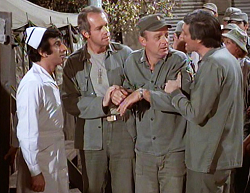
\includegraphics[width=\figwidth]{pics/14/32.png}
	\end{center}
\end{wrapfigure}
The only reason Doc didn't immediately panic and do something stupid, was that Gravis chose that exact moment to try and die again. 
The nurse ran over to assist, and Doc began barking orders at, for lack of anyone else, the two Security officers. 
Now Doc may not have been a REAL doctor, but he'd gotten quite good at keeping Sergeant Gravis alive over the last few weeks, and that medical confidence infused his voice with doctorly gravitas. 
The two Security officers stood there in shock for a second, and then, compelled by the voice of medical authority and the sight of an honest-to-the-Emperor Space Marine (well, half of one) lying on the table, they lowered their weapons and began helping too.

Now in an ideal galaxy, after they helped him save Gravis, Doc would've sent the two Security goons off on some pointless errand, and they would've spent hours running around looking for a cans of headlight fluid or elbow grease before remembering that they were supposed to be arresting him. 
What actually happened though, was that halfway through the procedure, a whole mob of people burst into the storage room. 
Only three of the intruders were Security grunts, the rest consisted of the other nurse, Sister Valerie, the Station's head medicae, and a very-angry looking man who turned out to be the head of the medbay Security detachment. 


The room was immediately filled with yelling, as the Security Commander started chewing out his men for swabbing the traitorous heretic's brow instead of arresting him, and the two men tried to defend their actions. 
At the back of the group one of the newly arrived goons began relaying a report to headquarters, another called for backup from the other search parties. 
The third goon was stuck trying to placate the head medicae and Sister Valerie, who were angrily demanding to know what all this talk of heretics and arresting was about. 


\begin{wrapfigure}{O}{\figwidth}
	\begin{center}
		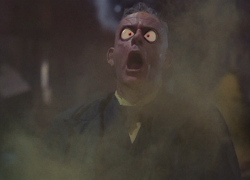
\includegraphics[width=\figwidth]{pics/14/33.png}
	\end{center}
\end{wrapfigure}
After a half a minute of trying to get information out of the low-level Security officer, Sister Valerie turned to the irate Commander, and tapped him on the shoulder. 
The Commander, who was still busy shouting at the men who'd been helping Doc, responded with a rather rude remark, then ignored her. 
This was what we in the Guard call a "Tactical Error". 
With a little huff of annoyance, Sister Valerie jammed an injector into the Security Commander's neck, and stalked past him with her nurse in tow. 
Behind her, the Commander rocked from side to side, then crumpled to the floor. 
In the silence that followed, Sister Valerie shooed Doc away from Gravis, and said she'd take care of the Space Marine while Doc dealt with "all this silliness".

Doc turned around and found himself facing a very shocked head medicae, and three Security officers who didn't quite have their weapons raised, but were obviously very angry. 
He briefly evaluated his chances of talking his way out of the situation, decided they were rather low, and raised the turkey-baster sized metal syringe full of fluid he'd just drained from Sergeant Gravis' Oolitic Kidney in the least-threatening way he could manage. 
Then, in a surprisingly swift motion, Doc jammed the syringe's plunger down, and hosed all three security troopers with Tyranid biotoxin.

The results were not pretty. 
None of the Security officers had their faceplates lowered, and Doc managed to nail two of them right in the mouth. 
They were the lucky ones: 
it only took them a few seconds to die, the third officer got hit in the eyes, and took nearly a minute. 
Sister Valerie looked up disapprovingly at the screaming, and pointed out that what Doc had just done was both distracting and terribly unhygienic. 
Doc stammered an apology, both to the Sister and to the three dead Security officers, then turned to the two officers who'd been assisting him, and were now backed as far away from him and his syringe as possible.

\begin{wrapfigure}{O}{\figwidth}
	\begin{center}
		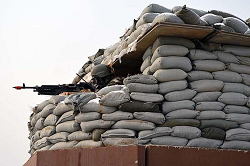
\includegraphics[width=\figwidth]{pics/14/34.png}
	\end{center}
\end{wrapfigure}
After a few seconds of thought on the ethical and tactical problems raised by the whole hostage thing, Doc told the two terrified Station Security officers to collect their unconscious commander, as well as the catatonic-with-fear head medicae, and get the hell out. 
Then, at Sister Valerie's insistence, he also shoved the three now-melting corpses out into the hallway. 
As an afterthought, he collected the dead officers' shotguns and ammo, set up a firing position using the sliding door and the sturdiest crate he could find, and thanked the Emperor that their storage room was at the end of a corridor. 


It should be noted, just for posterity, that Doc did NOT actually stop to check what was in the crate he used for his barricade. 
That really wasn't his fault though: 
he was very busy with defending the room, it was an innocent mistake, and the Tribunal DID clear him in the end.

Anyway, as Doc worked, he did his best to bring Sister Valerie up to speed. 
She did not find the news that the Astropaths had betrayed us surprising, and recommended purging them all in holy fire before we left. 
Doc made that agreeing, but noncommittal sound which comes naturally to all boyfriends, and skipped ahead to the part where they needed to pack everything back up and hold out until backup arrived. 
Since by this point the Security reinforcements had arrived and needed to be continually discouraged from advancing down the corridor, Doc was put on barricade duty, while Sister Valerie and her minions handled the packing and keeping Gravis alive.

\begin{wrapfigure}{O}{\figwidth}
	\begin{center}
		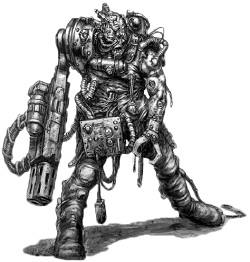
\includegraphics[width=\figwidth]{pics/14/35.png}
	\end{center}
\end{wrapfigure}
For the most part, between his entrenched position, the natural killzone, and his large supply of shotgun ammo, Doc didn't have that much trouble holding off Station security. 
It fact it wasn't even what you could really call "holding off", it was mostly a matter of popping a shot off whenever someone peeked around the corner at the end of the hallway and shooting down the odd servo-skull. 
The Security officers that had been guarding the medbay weren't die hard soldiers, they were just a police force, and their willingness to die gloriously for their station was rather lacking. 
Especially after some them tried to rush Doc using a makeshift boarding shield, and got pegged with a home-made tox grenade (really just a glass jar filled with more Tyranid biotoxin). 
Seeing half a dozen of your more gung-ho comrades die screaming and MELTING can really sap a man's enthusiasm.

Unfortunately, this happy state of affairs didn't quite last long enough. 
Right as Aimy's team was drawing close to medbay, and had switched from blitz to stealth mode, the Stationers found their spines and launched another serious attack. 
Or to be more precise, they found a pair of gun servitors. 
We all heard Doc start swearing over the comms as the servitors opened up with a pair of heavy stubbers each, and started shambling up the hallway while something like a dozen Security goons followed a few meters behind.

Doc made a good showing by all accounts, but the odds were stacked too high against him, and he was quickly forced to abandon his firing slit. 
As the servitors drew into close range, he took a gamble and used his last tox grenade. 
He got a bullet in the arm for his trouble, but at least it was AFTER he threw the grenade. 
The jar of Tyranid biotoxin hit it's mark, and quickly turned both servitors' fleshy bits into mush. 
Unfortunately, as the saying goes "If the enemy is in range, so are you", and several of the Security troopers had brought concussion grenades. 


\begin{wrapfigure}{O}{\figwidth}
	\begin{center}
		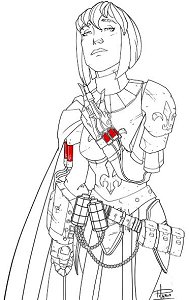
\includegraphics[width=\figwidth]{pics/14/36.png}
	\end{center}
\end{wrapfigure}
The entire barrage of grenades went off directly in front of the door to the storage room. 
The shockwave bent the door inward, ragdolled Doc across the storage room, and left him pinned under the heavy crate he'd been using as a barricade. 
He was pretty definitely out of the fight at that point, but luckily, Sister Valerie was there to rescue his sorry ass.

Now this is where things get a little fuzzy, because Doc was concussed, mostly deaf, bleeding both internally and externally, and is the very definition of a biased witness where his girlfriend is concerned. 
According to him, she calmly instructed her minions to finish packing, pulled a crate off the mobile medical suite, and kneeled down in front of it. 
Then, head bowed in prayer, she extracted Sergeant Gravis' Astartes Mark Vb Godwyn Pattern Bolter, and started glowing with the Divine Light of the Emperor.

We know this next part was bullshit, because Sister Valerie couldn't carry a tune with a bloody wheelbarrow, and had actually been banned, very politely mind you, from participating in the choir during the Occurrence Border's morning services. 
But Doc insisted that as she rose to her feet surrounded by a halo of divine light, and started singing a battle-hymn so divinely beautiful that it was painful. 
Then, a-singin' and a-glowin' like a bloody angel, she walked over to the door, and began mowing down wave after wave of Security goons with Gravis' bolter.

Now, we saw that hallway afterwards, and there definitely weren't enough bodies to constitute even a single wave, but we couldn't deny that she sure as hell shot the place to shit. 
She must have put at least three magazines of Astartes-sized bolt rounds down that hallway, though "down" really isn't the right word: 
the vast majority of the bolt-craters we could see were along the corridor's walls, ceiling, floor, and somehow even the door behind her. 
She had about as much control over that weapon as a toddler trying to walk a fenrisian wolf.

\begin{wrapfigure}{O}{\figwidth}
	\begin{center}
		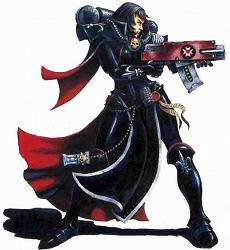
\includegraphics[width=\figwidth]{pics/14/37.png}
	\end{center}
\end{wrapfigure}
Lack of actual aiming ability aside though, Sister Valerie's counter attack got the job done. 
The sight of a tall blond bombshell incoherently screaming a Sororitas Battle Hymn, and firing what amounted to a fully automatic rocket launcher with all the accuracy and discipline of an enraged Ork was more than the Station Security troopers could handle. 
They ran for it, and when she kept shooting, they ran some more; 
if the medbay hadn't already been evacuated by the head medicae it would have been a lethal stampede, but as it was, the whole thing was just comical. 
The retreat ended with the whole cowardly lot sitting in the lobby, yelling at each other, and trying to explain the situation to their superiors and the newly-arrived reinforcements.

By this point those of us who'd been in the warehouse had navigated into an unoccupied maintenance corridor adjacent to the lobby, and were performing recon using Spot 2.0 and Fumbles. 
Seeing the idiots run out like there was a bloodthirster on their heels struck as hilarious, and it got even better when they told the reinforcements what had happened: 
in their terrified little minds Doc had grown into some sort of Nurglite mega-cultist. 


We caught phrases like "What sort of hell plague melts BONES?", "turned a sister of battle into a daemonhost", and "came here to resurrect his Plague Marine master". 
It was good stuff, really lightened our moods, and on a more practical note, the horror stories had completely drained the Security troopers' enthusiasm. 
They pretty much unanimously decided to just defend the lobby, and wait until one of the Station's SWAT teams arrived. 
This was good news for Doc, who was in no condition to fend off another attack, but it left the rest of us with the problem of getting him out past thirty-ish Security troopers before their heavies arrived. 
Luckily, Sarge had sorted out his issues by then and we were not forced to go with Tink's or, Emperor forbid, Nubby's proposed solutions.

\begin{wrapfigure}{O}{\figwidth}
	\begin{center}
		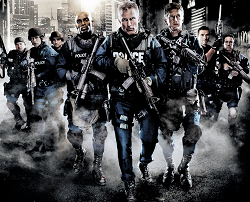
\includegraphics[width=\figwidth]{pics/14/38.png}
	\end{center}
\end{wrapfigure}
Sarge's defense of the Office Suite was not as exciting as Doc's desperate holdout, this was largely because the Stationers knew Sarge was incredibly dangerous form the beginning, and didn't bother sending a few waves of poorly trained Security officers to their deaths. 
Instead, they called for the Station's best SWAT team, and set about fortifying the entire Telepathica headquarters to prevent any chance of escape or rescue.

This sounded very bad to Sarge and the Diplomacy Adept, and they shared that opinion with Jim, who didn't respond except for fending Sarge off when he attempted to un-jack the tech-priest's mechadendrite from the comm terminal. 
There was a brief debate over whether he was okay, and if the "try and cut into a maintenance shaft" plan should be performed yet. 
Since the Cogitator Adept said that Jim was, for lack of a better word, talking with over fifty other tech-priests, Sarge decided to keep waiting, and set about fortifying the two-room suite. 
Then, once he'd reached the point where the suite was as fortified as physically possible, he commed Twitch for some advice, then fortified it even more.

At about the same time as Doc was wantonly employing Tyranid bioweapons against three unsuspecting Security officers, the SWAT team finally launched their assault. 
Eight men, armored in matte black, void-sealed carapace armor and wielding the best automatic shotguns the Administratum could requisition, silently entered the main conference room and took up positions covering the door to the suite. 
One of them carefully opened the door's control panel, found the emergency override, and began counting down.

At zero the door slid open, but did not reveal the group of desperate heretics they'd been expecting. 
Instead, all that was on the other side of it was the sheer metal surface of the suite's table, and a lumpy object the size of a basketball, which had been wedged against the door, and fell into the main conference room as it opened.

\begin{wrapfigure}{O}{\figwidth}
	\begin{center}
		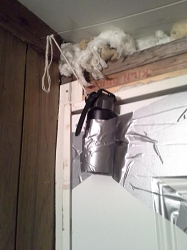
\includegraphics[width=\figwidth]{pics/14/39.png}
	\end{center}
\end{wrapfigure}
If the SWAT team'd had to time to inspect the object, they would've discovered that it consisted of six laspistol powerpacks, every extraneous metal skull, buckle, and stud that Sarge could rip off his Inquisitorial Costume, and few layers of duct tape. 
They didn't have time to inspect it though, because half a second after it hit the floor, the improvised frag mine went off and killed half of them.

On the far side of the massive pile of furniture, appliances, and bathroom fixtures that kept the table wedged against the door, Sarge felt incredibly relieved that the IED had worked like Twitch said it would. 
He raised his voice, and over the pained yelling of the two troopers who'd only been injured by the blast, Sarge told the survivors to bugger off. 
They responded by shooting the barricade a few times in a sort of desultory way, and then grabbed their wounded comrades and followed his advice.

Now, if it had been a Guard commander who'd just had his assault foiled like that, he would've said something like "Hmm, after killing so many of my men they must be low on ammo now, lets try that again", and Sarge would've been in deep shit. 
Fortunately the people in charge were just civilians, and even better, they were a committee; 
when the SWAT team's survivors limped back to them, they sat down and had a nice lengthy debate about what to try next. 
Sarge and the Diplomat listened in as idea after idea was raised and vetoed, usually for boring reasons like immense potential risk to personnel and property, but occasionally there was something more interesting. 
Apparently the Stationers were having a little trouble with their comms and cogitators, and no one from Mechanicus was returning their calls.

\begin{wrapfigure}{O}{\figwidth}
	\begin{center}
		
\includegraphics[width=\figwidth]{pics/14/40.png}
	\end{center}
\end{wrapfigure}
Eventually though, the committee reached a decision, and unfortunately, it was a pretty good one. 
The Telepathica knew enough about their own headquarters' to get into the ventilation system without a tech-priest's help, and the Shipmasters' Union was able to furnish several canisters of sedative gas. 
Once Sarge and his heretical companions were incapacitated, they'd send in some men with lascutters and rebreathers, and that would be that.

Sarge immediately taped up every vent he could find, but did not feel especially confident in the ability of a single layer of duct tape to fend off a chemical attack. 
His nerves began to fray as he overheard the gas being delivered then sent off to be deployed, and Jim still hadn't moved. 
The only thing that kept him from just forcing the tech-priest to wake up and trying to cut through the wall with his last two power packs, was the old Diplomat's calm assurance that he'd lose consciousness long before Sarge would, and could be used as a sort of final warning. 


Luckily, though it didn't seem so at the time, it never came to that. 
Right as the elderly adept started feeling woozy, Sarge noticed the telltale hum of a lascutter and a spot on the wall of the partially flooded bathroom began to glow. 
Sarge spared a few seconds to curse the Stationers for not mentioning that the assault was starting within the bugs' pickup range, then got ready to go down fighting. 
As a sort of afterthought he gave Jim a whack upside the head, partially to try and wake the him up, but mostly because he was rather angry with the enginseer. 
Jim didn't snap awake though, this was because he was already awake, and was in the process of turning around when Sarge swung.

The end result was Jim sitting on the floor, checking if his nose was broken, and calling Sarge some very unkind words. 
Sarge responded with a few choice insults on his own, but stopped when Jim pointed out that he was being very ungrateful for someone who'd just been rescued.

\begin{wrapfigure}{O}{\figwidth}
	\begin{center}
		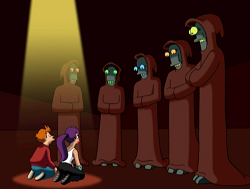
\includegraphics[width=\figwidth]{pics/14/41.png}
	\end{center}
\end{wrapfigure}
When the lascutter finished its work on the bathroom wall, the breach wasn't kicked open by a squad of heavily armed men. 
Instead, the precisely cut piece of metal drifted backwards then disappeared up the red-lit shaft on the other side, revealing a small swarm of servo-skulls. 
Sarge eyed the skulls with the special type of suspicion he reserved for anything that could be called "good luck", but Jim assured him they were friendly, and led the way into the shaft. 
As the enginseer entered, the skulls swarmed around him, and carefully lowered him down the shaft. 
Sarge noted that none of them had stuck around to lower him, hefted the woozy Adept under an arm, and slowly began descending the ladder at the back of the shaft. 
Up above him, a few skulls began welding the shaft closed again.

After a very long and slow climb, Sarge found himself in what was obviously a Mechanicus shrine, and flinched as he realized that he was surrounded on every side by tech-priests. 
The cogboys didn't seem hostile though, so Sarge just stood still and tried not to look like someone who endorsed tech-heresy in his subordinates. 
After a few seconds of motionlessness, Sarge noticed that none of the tech-priests were actually looking at him, and followed their gazes to where Jim was chirping in binary at what had to be the local Magos.

Jim's talk with the Magos went quickly, which was good, because Sarge was getting very tired of not being told what was going on. 
When Jim came over, Sarge got as far as "Just what the hell did you-" before the old Diplomat kicked him in the shin and suggested that he just let Jim take the lead. 


\begin{wrapfigure}{O}{\figwidth}
	\begin{center}
		
\includegraphics[width=\figwidth]{pics/14/42.png}
	\end{center}
\end{wrapfigure}
Using a haughty tone of voice that definitely didn't fit him, Jim began spouting a bunch of stuff about jurisdictions, re-prioritizations, and other such weasel words; 
it was complete bullshit, but luckily, Sarge was fluent in bullshit. 
The gist of it was that Jim had told the cogboys that he and Hannah had been given a vitally important mission by the Ordos Juris, and namedropped the two Magi that we'd so memorably encountered. 
This was, of course, a VERY creative interpretation of being told "go gain experience in the Inquisition, and we'll recruit you into the Ordos Juris if you survive", and Sarge took a small amount of pride in how much a cynical lying bastard Jim had become.

The local tech-priests couldn't directly assist with Jim's mission without knowing what it was, or being given some sort of authorization from higher up, but they could definitely help him return to his ship. 
Furthermore, if he made sure it didn't threaten the Station, they could make sure that said ship would be able to leave the system without being attacked. 
This was great news, but Sarge couldn't help but notice that only Jim and Hannah's escape and safety were mentioned, and pointed that out. 
Jim actually smiled a bit at that, and explained that the cogboys had no interest in us AT ALL unless we did something to significantly damage the Station. 
They'd wouldn't help us, but they wouldn't help the Stationers either, and they wouldn't do anything to stop us from following Jim on his very-safe trip back to the Occurrence Border through the Stations maintenance corridors.

In the end, Sarge sent the Diplomacy Adept off with Jim, but didn't go with them, because the Doc situation was heating up and Twitch was handling things just fine by himself. 
As they headed off, one of the tech-priests grudgingly showed Sarge to the nearest public corridor, then slammed the door behind him.

\begin{wrapfigure}{O}{\figwidth}
	\begin{center}
		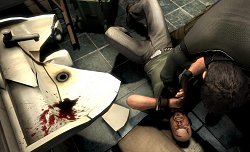
\includegraphics[width=\figwidth]{pics/14/43.png}
	\end{center}
\end{wrapfigure}
Sarge was now standing in a sparsely populated public corridor, wearing a ragged Inquisitorial Costume and a Evil Goon Uniform, which drew the eye better than a neon sign. 
Remembering the whole massive bounty on his head and station-wide arrest order thing, he ducked into to first unlocked door he could find, which luckily turned out to be a public restroom. 
He immediately stripped down to his skivvies and shoved the gaudy clothing into the nearest bin, then commed the cogitator Adept and set to work getting a less-conspicuous costume.

While he waited in the moderately filthy public restroom, Sarge listened to reports from the rest of us, and slowly formulated the most cunning of plans. 
A few minutes later, at about the same time as Doc was getting rescued by his girlfriend, a smalltime merc, who'd accepted a contract to remove an annoying drunk from a public restroom, opened the door and got one hell of a surprise. 
Sarge was very gentle by his standards, so the merc would probably live, though he probably wouldn't ever look at a toilet the same way again.

Atired in a bad-fitting, not to mention rather damp and smelly, merc uniform, and wielding a shoddily made Stationer shotgun, Sarge stepped out into the public corridor, and started jogging. 
A short distance away, two dozen mercenaries and bounty hunters entered a small dingy bar and looked around for the man that, according the comm messages they'd all received, had a lucrative contract for them.

\begin{wrapfigure}{O}{\figwidth}
	\begin{center}
		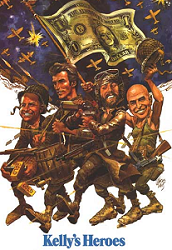
\includegraphics[width=\figwidth]{pics/14/44.png}
	\end{center}
\end{wrapfigure}
Now, it's been said, by just about everyone who's Sarge, that in the entire history of the Imperium there's been no one so inherently a Sergeant as him. 
He was born for it, destined for it, it was if the Emperor reached down and said "This guy, right here, he's going to be biggest, baddest, most sergeanty guy ever, and nothing can ever change that." He just sort exuded sergeant-ness, and anyone with a drop of military blood in their veins noticed it immediately. 
Well, as Sarge entered that bar full of mercs, he turned that aura up to eleven.

Sarge came through the bar door looking, despite his slovenly uniform, like he'd just stepped off recruiting poster, and every man in that bar, including the bartender, came to attention. 
Sarge surveyed them for a few seconds, then announced that he knew where the heretic bounties were hiding, and that Station Security was too chickenshit to handle them. 
He'd called them here, because they were toughest, meanest, nastiest men on the station, and if they followed him into this fight, they'd also be the richest. 
Then Sarge turned on his heel, and marched back out of the bar. 
The mercs, bounty hunters, and assorted scum in the bar all shared a look, then stampeded after him.

A short while later, Sarge and his small mercenary army shoved their way into the medbay lobby and demanded to speak to the commanding officer. 
Unfortunately, the security commander, who turned out to be the guy Sister Valerie had tranqued, was a bit less credulous than the mercs had been. 
He demanded to know who Sarge was (and no "Sarge" is not a name, it was a rank, what's your NAME merc?), what outfit he was from, and why he was there. 
Sarge, who knew from experience that claiming to be "Sergeant Sargent" would result in a fair bit of wasted time, discreetly checked the name on his ill-fitting jacket, and announced the he was Sergeant Kelly, the men behind him were Kelly's Heroes, and they were there to get rich or die trying.

\begin{wrapfigure}{O}{\figwidth}
	\begin{center}
		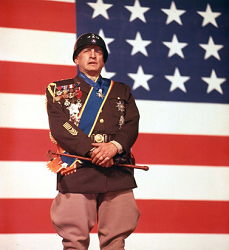
\includegraphics[width=\figwidth]{pics/14/45.png}
	\end{center}
\end{wrapfigure}
It took Sarge a bit of arguing to convince the Security Commander to let him launch an attack instead of just waiting for the Station's second-best SWAT team, but he managed. 
It helped a lot that, despite the fact that the Commander hadn't heard of any outfit called "Kelley's Heroes", the databases at Security HQ had. 
It turned out that it was an accredited mercenary company, which was in good standing with the Administratum, Telepathica and Shipmaster's Union, and it just happened to specialize in dealing with heretics. 
Imagine that!

Anyway, Sarge convinced the man to let him lead an assault on Doc's position, which meant that he had a nice excuse to get up on a table, and start giving a loud, impressive, and rather overlong heroic speech. 
Every man in the lobby turned their attention Sarge as he stomped back and forth, talking about bravery and valor, and all sorts of other heroic bullshit. 
No one noticed as a young man in a rumpled psyker's jacket sidled through the lobby's front door, around the edge of the audience, and into the hallway which everyone was supposed to be watching. 
They also completely failed to notice Spot 2.0 zipping in and out of the room, but since Spot was invisible this was far less of an achievement.

As Sarge's speech began to run uncomfortably long and the audience started to fidget, he received confirmation that everything was ready. 
He banged the table with the flagpole that he'd gotten from somewhere or other, and launched into the final, get-everyone-pumped up, part of the speech. 
Everyone's attention was neatly recaptured, which was good, because while they might have missed the large blurry shape that entering the from hallway, it would've been hard not to notice when it turned into Fumbles and the medical convoy and all the potted plants in the room withered. 
Luckily, after that little stumble, the convoy faded again, and no one noticed as it moved to the far corner of the lobby, where the wall was glowing slightly.

\begin{wrapfigure}{O}{\figwidth}
	\begin{center}
		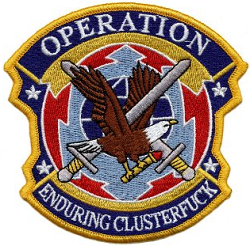
\includegraphics[width=\figwidth]{pics/14/46.png}
	\end{center}
\end{wrapfigure}
Sarge's speech ended with a final bellow of "CHARGE" and every man in the room, both the mercs and the security officers, surged towards the hallway that led to the now-empty storage room. 
Sarge didn't go with them though, as soon as they turned, he covered his eyes and bolted for the lobby's door. 
Up on the ceiling, Spot pulled a few pieces of string that had been run through the rings of a dozen flash and smoke grenades, and right as Sarge hit the doors, the lobby exploded into light and smoke. 
In the confusion, which quickly grew deadly as nearly fifty armed men panicked, no one noticed a section of wall collapsing, or the large blurry shape going through it.

Sarge stumbled through the lobby doors, feeling rather proud of how well that had worked out, and nearly collided with eight men in matte black armor. 
He froze for a second, resisted the urge to raise his shotgun, and told them that a bunch of heretics disguised as mercenaries had just attacked the Security forces. 
The leader of the SWAT team swore, and led his men through the doors. 
Sarge waited until the last one had gone through then sprinted like hell. 
As he reached the end of the hallway, a side door slid open to reveal Aimy, and somewhere behind him someone yelled "HEY YOU". 
Something stung Sarge in the side as he ran the last few meters to the door, and Aimy responded by leaning out and neatly putting a bolt of plasma through the offending SWAT trooper's helmet; 
then both of them were through the door.

Despite the fact the SWAT team following them had a nice clear trail of Sarge's blood to follow, they didn't manage to catch up. 
This was primarily because Aimy kept shooting the control panel of every automatic door after she closed it, but also because any Guardsman worth his salt is a good runner. 
Before long they reached the rest of us, Sarge was tossed onto the loot pallet next to Doc, and the whole convoy rolled out.

\begin{wrapfigure}{O}{\figwidth}
	\begin{center}
		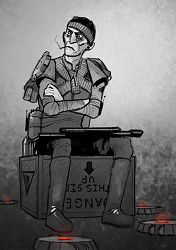
\includegraphics[width=\figwidth]{pics/14/47.png}
	\end{center}
\end{wrapfigure}
The trip across the station went surprisingly fast, and without incident. 
We later found out that this was because the Station's tech-priests were clearing the way for us by redirecting servitors and menials, and making sure every door was open. 
Apparently Jim had convinced them it was the best way to get us to stop cutting through things with Tink's plasma gun. 
Unfortunately, they hadn't been able to do anything to convince Twitch to stop being Twitch, and as we got closer to the the west dock, the signs of battle damage mounted.

Really though, anyone who knew anything about booby traps could tell that Twitch had been following Sarge's order to keep the body count low. 
There were a lot bloodstains, and the odd bodypart, but for the most part they were in the hallway leading towards the craters, as opposed to scattered around them. 
This was a clear sign of traps designed to act as deterrents instead of being set up for maximum casualties. 
Anyway, despite his restraint when it came to bodycount, Twitch and the ship's armsmen had really chewed the area around the docking bay up. 
It was a testament to the quality of the Station's construction that the entire section hadn't lost atmospheric integrity.

The mad bomber himself met us at the bottom of a freight elevator, flanked on either side by his last two suicide-skulls, and a pair of armsmen wearing the krootoid-spine necklaces that marked them as some of the tribals from hydroponics. 
The second we reached the elevator, the two skulls zipped away behind us, and we all felt a shockwave and heard the crash of a warehouse's worth of crates dropping into the corridor. 
Sarge briefly considered asking Twitch how many other corridors he'd collapsed, then decided that he really didn't want to know.

\begin{wrapfigure}{O}{\figwidth}
	\begin{center}
		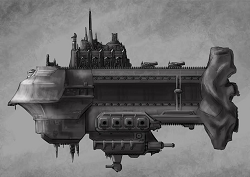
\includegraphics[width=\figwidth]{pics/14/48.png}
	\end{center}
\end{wrapfigure}
As we rode up the elevator Twitch brought us up to speed on how the defense of the Occurrence Border had been going. 
Apparently, largely thanks to the amount of flank Twitch's mines and skulls had been able to secure and the resulting terror in the attackers, it had gone very well. 
Casualties had been low, at least on our side, and the Captain had even been able to launch a small offensive to "liberate" some much needed supplies.

The only really bad development was that the Stationers had cut off the refueling pipe fairly early on, and no one had been able to figure out a way to steal any either. 
There was also the slightly worrying news that a few boarding shuttles had been launched by the Station. 
The few of these that had landed in the well populated sections of the ship were easily repelled by the armsmen, who had a rather significant home field advantage, but a few had landed in the tainted areas. 
Most of those shuttles hadn't taken off again, and Twitch predicted an increase in the amount of daemon activity until those poor bastards died and stopped feeding the things, but the two shuttles that had taken back off were almost more worrying. 
They'd landed in the Warp Fungus bay, so by now the stuff was probably already spreading through at least one of the Station's shuttle bays. 
Sarge commed Jim and asked him to send everything we had on the Fungus to the local cogboys, and we all hoped really hard that this wasn't going to turn out like the whole Necron thing: 
two sub-sector-wide disasters in a row would be really hard to explain to Oak.

After the elevator ride it was just a short walk through some blasted-open bulkheads to our docking bay. 
As we arrived, senior armsmen started bellowing orders, and an orderly retreat started. 
Twitch watched carefully as the men fell back, and began pulling color coded detonators off of his harness. 
One-by-one the abandoned defensive positions were demolished, and everyone filed back aboard the Occurrence Border.

\begin{wrapfigure}{O}{\figwidth}
	\begin{center}
		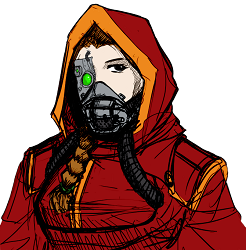
\includegraphics[width=\figwidth]{pics/14/49.png}
	\end{center}
\end{wrapfigure}
Once we'd boarded the ship, we split up again. 
Doc hobbled off with the medical convoy to get Gravis back into his old bed and either help out with the wounded, or get himself treated. 
The loot-pallet was taken down to the Psyker Holding Cells, though Nubby, Fumbles, and several boxes fell off along the way, leaving Aimy to help Tink, Fio, and Jim with all the unpacking. 
Twitch wandered off with his two tribal bodyguards to see about securing the entrances to the tainted areas. 
Finally Sarge, who wasn't quite wounded enough to be able to justify escape to the medbay, trudged up to the bridge to see how our escape was going.

Along with it's usual staff of interchangeable officers, the bridge was occupied old Diplomat, Hannah, and the Captain, and the Quartermaster. 
Sarge was struck by how calm the bridge was. 
He'd expected it to be as chaotic at it had been after first capturing the damned Zoanthrope, but the most exciting thing happening was an argument between the Captain and his quartermaster about the technical definition of piracy. 
Sarge noted that the Captain was nearly covered with blood, which couldn't have been his given that he was still standing, and the Quartermaster's augmetic arm had gone missing, and made a note to ask them how their escape from the Station had gone.

When Hannah noticed Sarge's arrival, she cut off her discussion with the Diplomacy Adept, marched over to him, and launched into an angry lecture about how he kept getting Jim into trouble. 
Sarge bore this with his usual stoicism, at least until the tech-priestess yelled at him for doing his "stupid servitor impression" and kicked him in the shin. 
As Sarge hopped around and cursed at her, Hannah stalked off the bridge, and the Diplomacy Adept took her place. 


\begin{wrapfigure}{O}{\figwidth}
	\begin{center}
		
\includegraphics[width=\figwidth]{pics/14/50.png}
	\end{center}
\end{wrapfigure}
After he finished laughing at Sarge's expense, the old Diplomat brought Sarge up date. 
Hannah had explained the Mechanicus' neutrality to the Captain, which is why the bridge wasn't in a panic. 
The Occurrence Border was headed out of the system, but since the tech-priests on the Station, as well as every ship in the system, were preventing the use of any anti-ship weapons, there was no need to rush. 
Sarge though this was a dangerously optimistic viewpoint, but didn't feel like arguing with Captain, and anyway, it meant that Tink and the rest would have more time to repair the Psyker Containment Cells.

Sarge was about to leave the bridge to see about having the buckshot removed from his side and changing into uniform that fit and didn't smell of urine, when the communication officer called him over. 
The Station was broadcasting a message, unencrypted and addressed to him by name of "The Heretical False-Interrogator Greg Sargent", which turned out to be a vid from the Station's leaders. 
Or more precisely, it was a vid from the Choir Master, the other two leaders mostly sat in the background and looked scared, and you couldn't really call it a message either. 
It turned out to be nearly twenty straight minutes of wide eyed ranting and death threats, which went from frightening, to amusing, to tedious, then briefly back to amusing when the enraged Astropath managed to break a blood vessel in his eye and had to be taken away to calm down. 


Unfortunately, the vid resumed after that, and the Choir Master shifted from pointless screaming to promises of vengeance. 
Among many other things, he vowed that every choir from Ultramar to Terra would hear of our crimes, which struck Sarge as a very petty and stupid form of vengeance. 
It'd cause immense annoyance the in the short term, but it would ensure that Inquisition found out, and get everything sorted out that much quicker. 


\begin{wrapfigure}{O}{\figwidth}
	\begin{center}
		\includegraphics[width=\figwidth]{pics/14/51.png}
	\end{center}
\end{wrapfigure}
Eventually, as the Choir Master ramped back up into ranting again, Sarge got bored. 
He told the communications officer to just send a copy to the Adepts, and declined when asked if he wanted to send a reply. 
Then, with a wave at the Captain and a promise to come up and help plan the route when the ship reached safe warp distance, Sarge left.

A few hours and a much needed nap later, Sarge headed down to the Psyker Holding Cells, and found them empty; 
just of people though, the Zoanthrope was exactly he'd left it, thank the Emperor. 
Sarge flipped the bug off out of habit, and checked the room down the hallway that had become Tink, Fio, and Jim had claimed as their break and nap room. 
He found the three nerds, accompanied by Hannah, sitting around a screen, watching their usual vile Tau vids. 


Sarge eyed Hannah warily, but the cog-girl did not seem inclined to violence at present, so he advanced into the room and prodded Tink. 
At first the techie refused to answer questions, but after Sarge threatened to break the vid player, he became a bit more helpful. 
Tink confirmed that everything in the Cells was working fine, they hadn't had the raw materials to just rebuild the cells like they'd wanted, but Nubby had gotten all the crucial repair parts. 
Everything should hold together fine for at least two weeks of warp travel, which was more than enough time to reach a less-crazy Imperial outpost. 
Sarge recalled that cause of that craziness, and asked what the odds were of another Astropath killing psychic explodey thingy. 
He got a lot of technobabble, which he assumed meant "we're not really sure why that happened, but it probably won't happen again".

\begin{wrapfigure}{O}{\figwidth}
	\begin{center}
		\includegraphics[width=\figwidth]{pics/14/52.png}
	\end{center}
\end{wrapfigure}
His curiosity sated, Sarge turned to leave the room, but paused as the something on the vid caught his eye. 
It was a fat man, wearing what Sarge recognized, thanks to some unwanted training on the subject, as Floral-Printed Tau formal robes. 
As the animated figure gibbered in Tau-speak, Sarge realized that he was looking at some bizarre caricature of ex-Inquisitor Lars Weebu, and with dawning sense of horror he realized what was going to come next.

There was a blast of shrill music, followed by a few lines of text which Sarge hesitantly translated as "Super Deserter Gue'vesa Action Heroes", and the scene change to a group of six characters wearing Tau flak armor. 
Sarge's eye scanned the horrible big-eyed characters for the telltales he knew would be there. 
There was the red cross on one, the bandoleers of explosives on another, and then there was the half-sized character with his psyker-robe wearing sidekick. 
At the back of the group he spotted a character with chevrons, who looked far grumpier and grayer than seemed appropriate, and finally there was… Well, it had the oversized plasma gun, and the goggles, and the drone, so it had to be… but...

"Umm, Tink, why… why is your character female?"

The techie froze, and slowly looked up at Sarge. 
Jim snickered.

"Ahh… w-well.. 
y-y-you see…" stammered Tink.

Fio, seeing that Tink was having trouble, decided to help. 
"That actually just happened, last week they were fighting the dread wych Ynageza and she cast a spell which-"

"FORGET I ASKED."
